% harryopo-slides 示例：作品路演（dark 主题）
\documentclass[dark]{harryopo-slides}
\title[知行读书]{知行读书：让每个读者都有一位 AI 书童}
\subtitle{创新大赛路演 · 2026}
\author{张三（CEO） \and 李四（CTO）}
\institute{知行工作室}
\date{2026年9月}
\begin{document}

\begin{frame}[plain]\titlepage\end{frame}

\begin{frame}{痛点：读完就忘}
\begin{itemize}
  \item \alert{87\%} 的读者两周内遗忘书中大部分观点
  \item 划线、笔记散落三个 App，无法汇聚成知识
  \item 现有 AI 摘要只会"缩写"，不会"教会你"
\end{itemize}
\note{开场用主持人给的数据，停顿两秒再翻页。}
\end{frame}

\begin{frame}{我们的解法}
\begin{block}{}
AI 书童 = 苏格拉底式提问 + 间隔复习 + 自动知识图谱
\end{block}
\vspace{0.8em}
\begin{center}
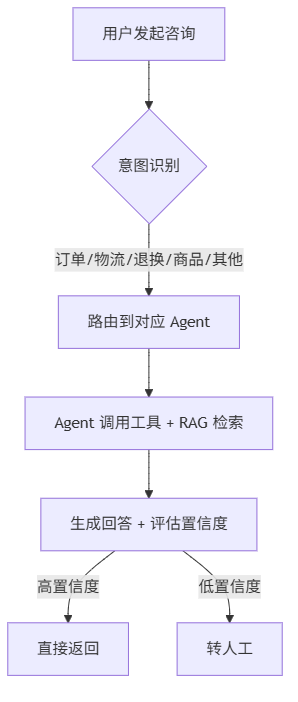
\includegraphics[width=0.55\textwidth]{figures/flow.png}\\[0.4em]
{\footnotesize 用户 → 编排引擎 → 智能体池 → 记忆系统}
\end{center}
\note{流程图讲三跳：提问、复习、沉淀。}
\end{frame}

\begin{frame}{市场规模}
\begin{columns}
\column{0.33\textwidth}\centering{\Huge\alert{480亿}}\\ 数字阅读市场
\column{0.33\textwidth}\centering{\Huge\alert{1.2亿}}\\ 年度知识付费用户
\column{0.33\textwidth}\centering{\Huge\alert{0}}\\ 直接竞品（空白赛道）
\end{columns}
\note{TAM/SAM/SOM 口径来自 2026 行业白皮书，附录有出处。}
\end{frame}

\begin{frame}{路线图}
\begin{enumerate}
  \item Q3：核心问答 + 微信小程序上线
  \item Q4：知识图谱与复习引擎（\alert{已内测 200 人}）
  \item 2027 Q1：开放平台，接入出版社书库
\end{enumerate}
\note{强调 Q4 内测留存数据：次日留存 61\%。}
\end{frame}

\begin{frame}[plain]
\begin{center}\vspace{2em}
{\Huge 让阅读真正发生}\\[1em]
{\normalsize 期待与你同行 \quad\textbar\quad 融资用途：研发 60\% / 内容 25\% / 运营 15\%}
\end{center}
\note{收尾，联系方式在附录最后一页。}
\end{frame}
\end{document}
